\section{Computação Clássica} 
Entende-se a importância de se compreender a origem e o desenvolvimento da computação clássica para o desenrolar da pesquisa, o que será apresentado em meio a este capítulo.

A computação clássica consiste em computadores que dependem da física clássica para operar. Estes são os computadores tradicionais que usamos em nosso dia-a-dia – seja eles Apple, Samsung, Dell ou qualquer outro –, também classificados como computadores binários, pois processam as instruções a partir de números binários, compostos apenas pelos símbolos “1” e “0”, ligado e desligado respectivamente. Assim, julga-se importante e de larga relevância ao tema compreender essa representação numérica. 

Números binários ou números em base 2 são compostos por apenas dois dígitos, [0...1]. Dessa forma, seu funcionamento é similar ao sistema decimal, ou base 10, que são compostos por dez dígitos, [0...9]. No sistema decimal, é simples contar até nove, porém não existe um simbolo ou dígito para representar o número dez, sendo então representado  dois dígitos, “10”. Isto é uma simples lógica de posicionamento. Mais uma vez, após o número “99”, é necessário utilizar a mesma regra para representar o número cem, “100”. Em base 2, o número zero é representado pelo simbolo 0, e o número um por 1. O mesmo dilema é enfrentado ao chegar no próximo valor, dois. E então é usada a mesma lógica de posicionamento, em base dois. O número dois é representado por “10”, o três por “11”, quatro por “100” e assim por diante. Dessa forma, números binários podem se tornar longos e compostos por muitos dígitos. Em computação, esses dígitos são chamados de bits. \cite{6} É com base nos \label{bits}bits\footnote{A menor unidade de informação que pode ser armazenada ou transmitida na comunicação de dados.} ligados e desligados que o computador baseia sua linguagem. Para transforma-lo em base dez é preciso avaliar o valor de cada bit de acordo com a sua posição. 

Exemplo: número binário $1011$:

\[ 1011(b) = 1*2^3 + 0*2^2 + 1*2^1 + 1*2^0\]
\[ = 8 + 0 + 2 + 1 = 11(decimal)\]

O peso de cada bit de um número binário depende da sua posição relativa ao número completo, sempre partindo da direita para a esquerda.

\begin{itemize}
  \item O peso do primeiro bit é $bit * 2^0$
  \item O peso do segundo bit é $bit * 2^1$
  \item O peso do terceiro bit é $bit * 2^2$
  \item O peso do quarto bit é $bit * 2^3$
\end{itemize}

A formúla ilustrada acima, pode ser exemplificada em uma fórmula genérica: 

\[= nth\: bit * 2^{n-1}\]

É possível notar que a regra para números binários, se repete para números em base 10.

Exemplo: número decimal $4392$:
\begin{itemize}
  \item O peso do primeiro bit é $2 * 10^0$
  \item O peso do segundo bit é $9 * 10^1$
  \item O peso do terceiro bit é $3 * 10^2$
  \item O peso do quarto bit é $4 * 10^3$
\end{itemize}
\[ 4392 = 4*10^3 + 3*10^2 + 9*10^1 + 2*10^0\]
\[= nth\: bit * 10^{n-1}\]

Essa regra se mantem verdadeira para qualquer base númerica.

\[= nth\: bit * (base)^{n-1}\]

Ao decorrer do texto serão referidos números em base 2, 10 e 16. 

\subsection{A computação clássica e sua evolução}
Alan Turing, Matemático inglês, cientista da computação, lógico, criptoanalista, filósofo e biólogo teórico, publicou o artigo “On Computable Numbers with an Application to the Entscheidungs-problem” \cite{8} em 12 de novembro de 1937, esse formaria a teoria básica da computabilidade por várias décadas.

O mecanismo abstrato descrito no artigo de Turing fornece os conceitos fundamentais de computadores que outros engenheiros conceberam posteriormente. Na sua essência, uma Máquina de Turing é um dispositivo que manipula símbolos em uma tira de fita de acordo com uma tabela de regras. Forneceu formalização dos conceitos de “algoritmo” e “computação” na infância da ciência da computação. Apesar de sua simplicidade, uma Máquina de Turing pode ser adaptada para simular a lógica de qualquer algoritmo de computador e é útil para explicar as funções de uma CPU.

Turing é identificado não apenas como o pai da ciência da computação, mas também como o pai do computador clássico. O fundamento para isso é o seguinte, o diagrama do computador moderno pode ser encontrada no projeto EDVAC de Von Neumann \cite{9} e hoje os computadores clássicos são geralmente descritos como tendo a chamada arquitetura de Von Neumann. Uma idéia fundamental do design do EDVAC é a idéia de programa armazenado. Isso significa o armazenamento de instruções e dados na mesma memória, permitindo a manipulação de programas como dados. Existem razões para supor que Von Neumann conhecia os principais resultados do trabalho de Turing \cite{10}. Assim, pode-se argumentar que o conceito de programa armazenado se origina da noção de máquina de Turing e, destacando isso como a característica definidora do computador clássico, alguns podem alegar que Turing é o pai do computador até o estado da arte. Outro argumento relacionado é que Turing foi o primeiro a explorar a idéia de uma máquina de uso geral por meio de sua noção de máquina universal e que, nesse sentido, ele também “inventou” o computador moderno. Esse argumento é reforçado pelo fato de que Turing também estava envolvido na construção de uma classe importante de dispositivos de computação, o Bombe \footnote{um dispositivo eletromecânico usado pelos criptologistas britânicos para ajudar a decifrar as mensagens secretas criptografadas pela máquina alemã Enigma durante a Segunda Guerra Mundial.}. Posteriormente, ele propôs o design do ACE (Automatic Computing Engine), explicitamente explicado. identificado como um tipo de realização física da máquina universal pelo próprio Turing:

\textit{
  ``Some years ago I was researching on what might now be described as an investigation of the theoretical possibilities and limitations of digital computing machines. […] Machines such as the ACE may be regarded as practical versions of this same type of machine.'' \cite{11}
}

Baseando na teoria da máquina de Turing, o físico e matemático John von Neumann desenvolveu uma arquitetura que era capaz de executar tais tarefas.

\begin{figure}[H] \centering 
  \makebox[\textwidth][c]{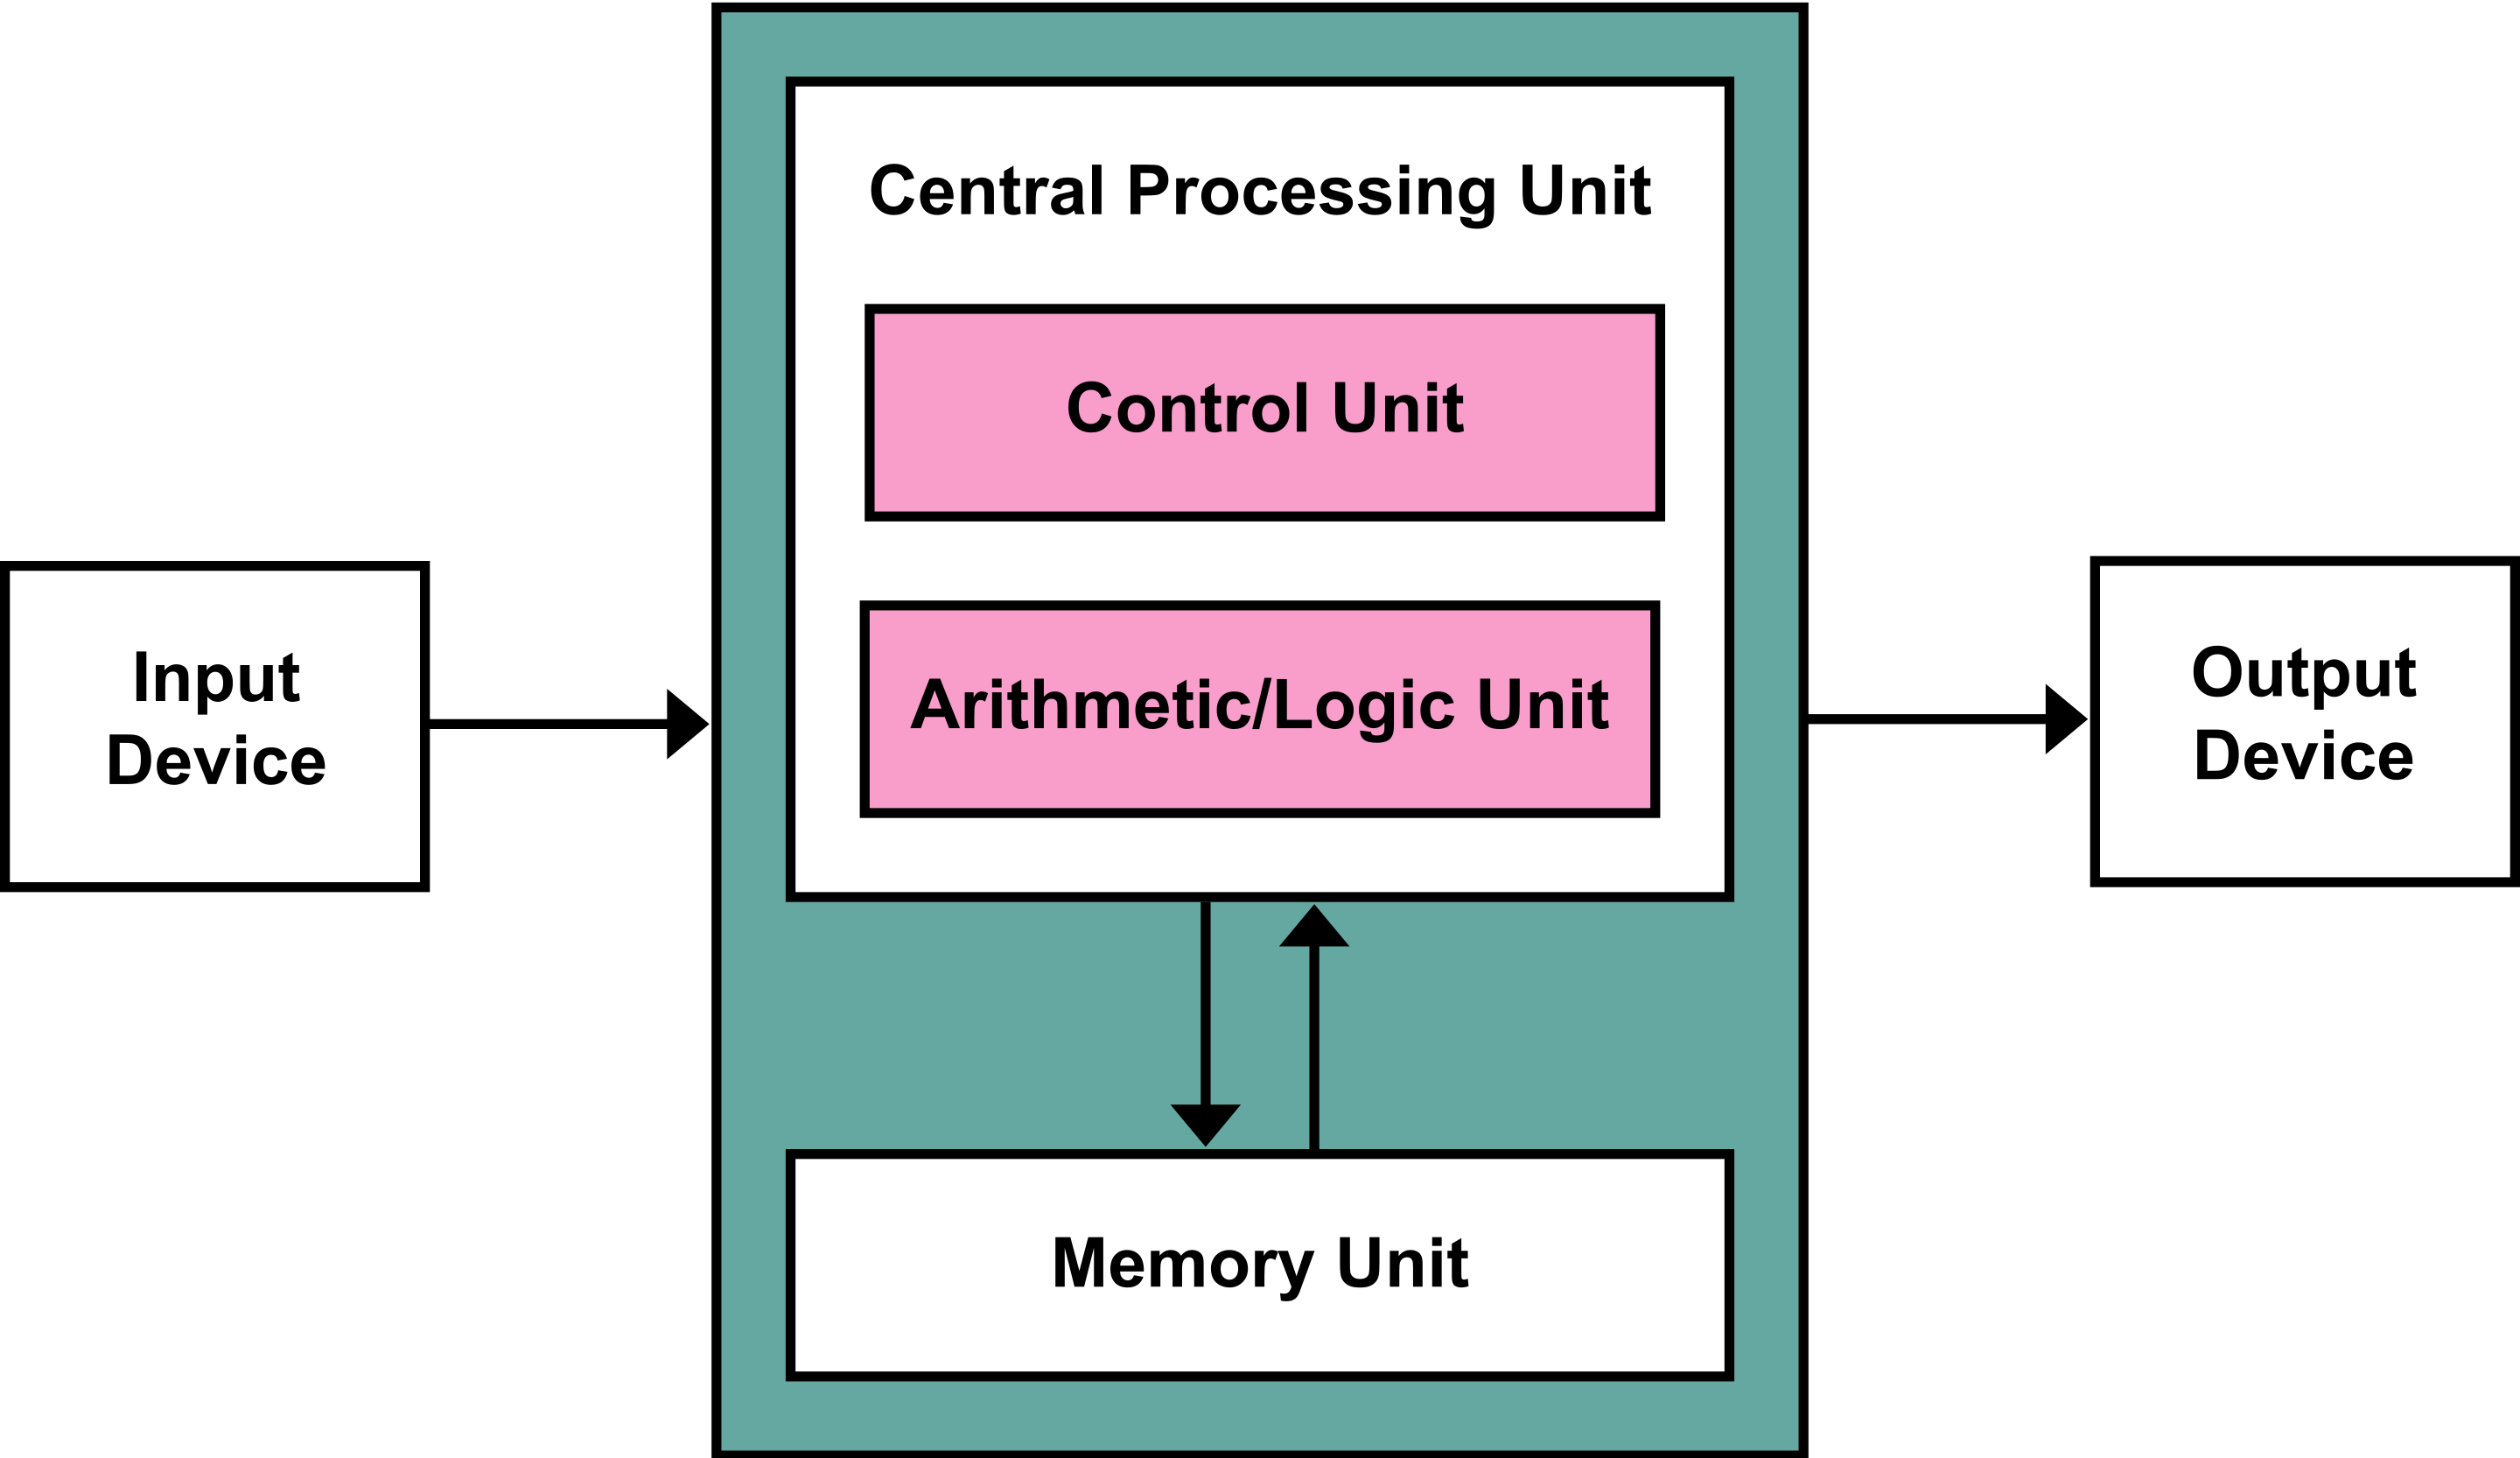
\includegraphics[width=0.8\textwidth]{von_neumann_architecture}}
  \caption{\label{fig:1} Diagrama arquitetura de Von Neumann} 
\end{figure}

Nessa arquitetura, o cabeçalho passa a ser uma CPU (Central Processing Unit), a fita se transforma em memória RAM e as operações são construidas e executadas em circuitos formados por portas logicas  chamado ALU (Arithmetic/Logic Unit). \cite{12}

Atualmente, a maioria dos computadores modernos são construídos sobre a praxis da arquitetura von Neumann. A fim de simular um processador moderno de forma didática, foi elaborado o \href{https://gzsig.io/vm-24bits/}{ASM 24bits} este apresenta as principais características de um processador moderno e permite a sua programação utilizando um Assembly de 20 instruções, sua \href{https://github.com/gzsig/Asm/blob/master/README.md}{Documentação}. Similar à arquitetura de von Neumann esse emulador é composto por memória e CPU.


\begin{tabular}{ |p{3cm}||p{9cm}|  }
  \hline
  \multicolumn{2}{|c|}{Registradores} \\
  \hline
    Nome &Descrição\\
  \hline
    Accumulator (ACC) &Este é o registro mais usado para armazenar dados extraídos da memória. Está em diferentes números em diferentes microprocessadores.\\
  \hline
    Instruction Register (IR) &É o registro que contém a instrução que está sendo executada atualmente.\\
  \hline
\end{tabular}

\newpage
